\documentclass[11pt,a4paper]{article}

\usepackage[margin=1in]{geometry}
\usepackage{amsmath,amssymb}
\usepackage{booktabs}
\usepackage{graphicx}
\usepackage{microtype}
\usepackage{tikz}
\usetikzlibrary{arrows.meta,positioning,fit,backgrounds,calc}
\usepackage{pgfplots}
\pgfplotsset{compat=1.16}
\usepackage{subcaption}
\usepackage[hidelinks]{hyperref}
\usepackage{natbib}
\bibliographystyle{plainnat}

\title{Content-Addressed Continual Memory with On-Demand Capacity}

\author{%
  Xinyu Yang\\
  \texttt{pana.yang@hotmail.com}\\
  ORCID: \href{https://orcid.org/0009-0007-2600-0948}{0009-0007-2600-0948}
}

\date{\today}

\begin{document}
\maketitle

\begin{abstract}
We study a continual-learning memory in which storage is addressed by content,
capacity is allocated on demand from the stream without task identifiers, and
new capacity is appended without perturbing anything already stored. On a
relational stream whose regimes are distinguishable from their inputs, the
mechanism retains $49.5\%$ of probed facts zero-shot against $15.1\%$ for a
monolithic sparse-coded control of the same width, which is itself at the level
of a linear baseline; the advantage narrows from $34$ to $25$ points between
eight and thirty-two regimes without closing. Sharing the payload transform
across regimes while keeping per-regime readouts adds $16.4$ points over a
fully private variant (six seeds, $p<0.001$). Allocating readout rows only for
targets a regime actually emits reduces occupied capacity by $7.6\times$ at no
cost in accuracy, and appending capacity leaves existing weights byte-identical
and existing predictions bit-identical.

We give equal space to what the mechanism does not do, and hold those readings
open rather than assert them. It carries nothing between facts beyond a
single-timescale context, and retention falls as a cue is separated from its
query; multi-hop routing occupies the same capacity for less accuracy, and
letting the address compose as well as the value costs more still; retention
declines as regimes accumulate, with capacity starvation, worsening misrouting
and failing separation each excluded by measurement, leaving retrieval
difficulty as the surviving account. We report these as measurements whose
interpretation is unsettled because, in the course of this study, six
measurements that read as findings turned out to have been produced by the
measurement rather than the mechanism.
\end{abstract}

\section{Introduction}

A learner that must absorb an unbounded stream with bounded parameters has to
discard something. Regularisation methods such as elastic weight consolidation
\citep{kirkpatrick2017overcoming} give up plasticity, protecting old weights at
the cost of new learning. Methods that simply keep training give up the past.
A third option is to \emph{allocate}: give distinct regimes distinct storage, so
that degradation is uniform rather than selective. Dynamically expanding
architectures \citep{rusu2016progressive,yoon2018lifelong} take this route and
are routinely criticised for adding parameters per task without demonstrating
that the addition is proportionate to new content rather than to task count.

This paper examines an allocation mechanism built around three commitments.
Addressing is by content through a fixed random hash, so a fact reaches the same
storage under every history. Regime identity is inferred online from the stream,
so no task identifier, task boundary, or replay buffer is required. Capacity is
appended rather than resized, so adding storage leaves what is already there
untouched, which we check exactly rather than statistically.

We report what these commitments buy and what they cost. They buy a large
advantage where regimes are distinguishable, a capacity footprint that follows
emitted content rather than vocabulary size, and a per-token cost independent of
sequence length. They cost the ability to associate items across a gap, which
content-only addressing forbids by construction, and they leave retention
declining as regimes accumulate.

\paragraph{Contributions.}
\begin{enumerate}
  \item An allocation mechanism whose two addressing factors --- content to a
  memory slice, inferred regime to a readout --- are separately measurable, with
  no task supervision at any point (\S\ref{sec:method}).
  \item Evidence that sharing the payload transform while privatising the
  readout is the effective split for a stream whose regimes share surface form and
  differ in targets, confirmed from both directions (\S\ref{sec:sharing}).
  \item A capacity result: sampling negatives from a regime's own emitted
  targets makes occupancy follow content, $7.6\times$ smaller at equal accuracy
  (\S\ref{sec:capacity}).
  \item A non-destructiveness property, verified exactly rather than
  statistically: appending capacity leaves stored weights and predictions
  unchanged bit for bit (\S\ref{sec:expansion}).
  \item Measurements of what the mechanism does not currently do --- cross-gap
  association, multi-hop addressing, and retention as regimes accumulate ---
  reported with the alternative explanations we could exclude, and left open
  where we could not (\S\ref{sec:open}).
\end{enumerate}

\section{Related work}

\paragraph{Continual learning.}
Catastrophic interference in distributed representations
\citep{mccloskey1989catastrophic,french1999catastrophic} motivates three broad
families \citep{parisi2019continual,delange2021continual}: regularisation
\citep{kirkpatrick2017overcoming}, rehearsal, and architectural expansion
\citep{rusu2016progressive,yoon2018lifelong}. Our mechanism is architectural,
but differs from prior expansion methods in that it requires no task boundary to
decide when to expand; the decision is made from the dispersion of an inferred
regime's own statistics. Task-free continual learning
\citep{aljundi2019task} shares this aim.

\paragraph{Conditional computation.}
Structurally the mechanism is a single-layer, top-1 sparsely-gated mixture of
experts \citep{shazeer2017outrageously,fedus2022switch} whose router is a fixed
random hash rather than a learned gate, and whose expert count grows. We treat
the unlearned router as a limitation to be reported rather than a feature: it
forgoes load balancing and learned specialisation, and it is precisely what
prevents context from influencing retrieval (\S\ref{sec:longrange}).

\paragraph{Addressable and distributed memory.}
Content-addressed storage with sparse codes follows sparse distributed memory
\citep{kanerva1988sparse} and hyperdimensional computing
\citep{kanerva2009hyperdimensional}. Recoverable association of \emph{pairs},
which a smoothed context summary cannot provide, is available through
holographic reduced representations \citep{plate1995holographic} or fast-weight
outer products \citep{ba2016using,schlag2021linear}; we identify this as the
missing ingredient rather than claim it.

\paragraph{Consolidation across timescales.}
Cascades of variables at multiple timescales
\citep{fusi2005cascade,benna2016computational} target the capacity--lifetime
tradeoff of bounded synapses. We tested such a cascade in two roles, as weight
consolidation and as input context, and report both outcomes.

\paragraph{Attention and its costs.}
Self-attention \citep{vaswani2017attention} pays $O(N)$ per token in context
access and degrades on material in the middle of long contexts
\citep{liu2024lost}. A content-addressed memory pays a cost independent of $N$;
we quantify the crossover in \S\ref{sec:cost}.

\paragraph{Vocabulary growth.}
That distinct types grow sublinearly in a Zipf-distributed stream is Heaps' law
\citep{heaps1978information}. We use it to ask whether allocated capacity
tracks content, and find that our generator does not reproduce the sublinear
regime, which makes it an unfavourable source for the question
(\S\ref{sec:capacity}).

\section{Method}
\label{sec:method}

\subsection{Notation}

Let $\mathcal{V}$ be the vocabulary, $V=|\mathcal{V}|$, and $d$ the code width.
The embedding table $\mathrm{E}\in\mathbb{R}^{V\times d}$ has rows drawn
independently and uniformly from the unit sphere $S^{d-1}$ at construction and
is \emph{never} updated; $\mathrm{E}_x$ denotes the row of token $x$. Write
$\nu(x)=x/\lVert x\rVert_2$ for $\ell_2$ normalisation and $\delta_t$ for the
indicator vector of token $t$.

Storage lives on a small-world ring $G=(\mathcal{N},\mathcal{E})$ with
$|\mathcal{N}|=n$ nodes: node $u$ has out-neighbours consisting of its two ring
neighbours plus a fixed number of random shortcuts, giving out-degree $D_u$ and
$|\mathcal{E}|=M=\sum_u D_u$ directed edges. Every edge $a\in\mathcal{E}$
carries two objects: a \emph{key} $\kappa_a\in\mathbb{R}^d$, drawn once at
construction and never updated, and, for each regime class $c$, a learned
matrix $W^{(c)}_a\in\mathbb{R}^{d\times d}$. Each class $c$ additionally owns a
readout $R^{(c)}\in\mathbb{R}^{V\times d}$ and a prototype
$\pi_c\in S^{d-1}$. The number of live classes $C$ is not fixed in advance; it
grows (\S\ref{sec:allocation}).

A fact is a triple $(e,r,t)\in\mathcal{V}^3$: entity, relation, target. The
stream is a sequence of tokens $x_1,x_2,\dots$ from which facts are read off,
seen once each in the order they arrive.

\begin{figure}[t]
\centering
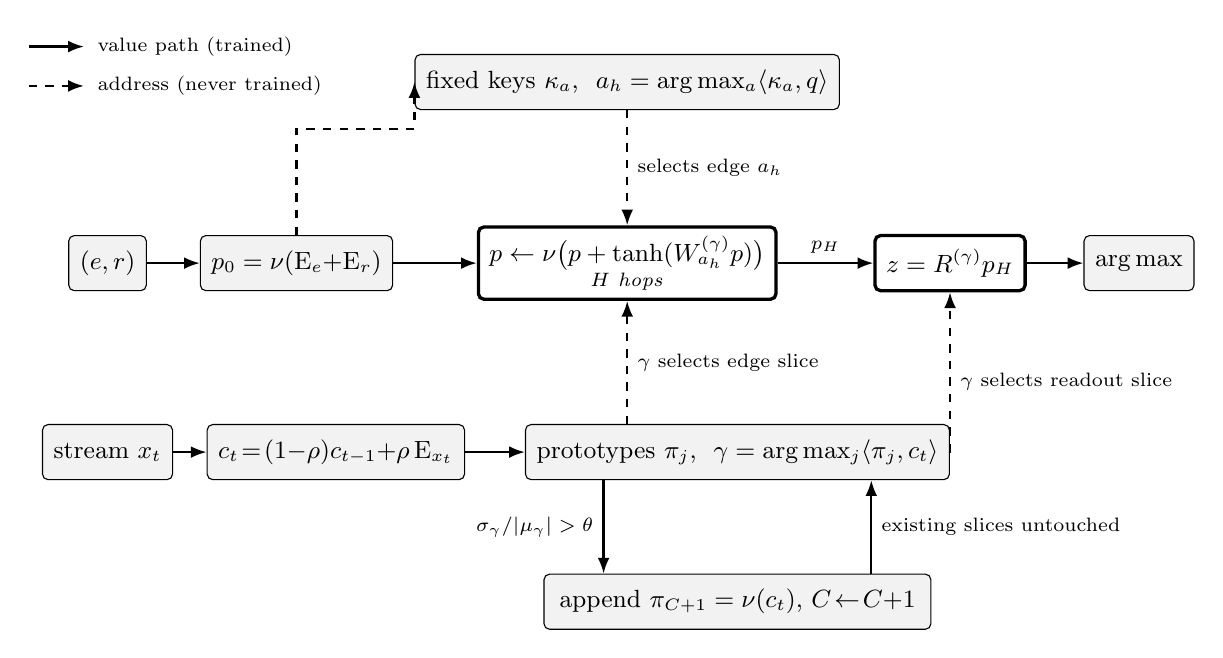
\begin{tikzpicture}[
  font=\small,
  box/.style={draw, rounded corners=2pt, minimum height=7mm, inner xsep=4pt, align=center},
  fix/.style={box, fill=black!5},
  lrn/.style={box, very thick},
  ar/.style={-{Latex[length=2mm]}, thick},
  addr/.style={-{Latex[length=2mm]}, thick, dashed},
  lbl/.style={font=\scriptsize},
]
% ---------- legend ----------
\draw[ar]   (-1.0,2.75) -- (-0.3,2.75);
\node[lbl,anchor=west] at (-0.25,2.75) {value path (trained)};
\draw[addr] (-1.0,2.25) -- (-0.3,2.25);
\node[lbl,anchor=west] at (-0.25,2.25) {address (never trained)};

% ---------- value path ----------
\node[fix] (er)  at (0,0)    {$(e,r)$};
\node[fix] (p0)  at (2.4,0)  {$p_0=\nu(\mathrm{E}_e{+}\mathrm{E}_r)$};
\node[lrn] (w)   at (6.6,0)  {$p\leftarrow\nu\big(p+\tanh(W^{(\gamma)}_{a_h}p)\big)$\\[-2pt]
                              \textit{\scriptsize $H$ hops}};
\node[lrn] (rd)  at (10.7,0) {$z=R^{(\gamma)}p_H$};
\node[fix] (out) at (13.1,0) {$\arg\max$};
\draw[ar] (er) -- (p0);
\draw[ar] (p0) -- (w);
\draw[ar] (w)  -- node[lbl,above]{$p_H$} (rd);
\draw[ar] (rd) -- (out);

% ---------- factor 1: content selects the edge ----------
\node[fix] (ring) at (6.6,2.3) {fixed keys $\kappa_a$,\ \ $a_h=\arg\max_a\langle\kappa_a,q\rangle$};
\draw[addr] (p0.north) -- ++(0,1.35) -| (ring.west);
\draw[addr] (ring) -- node[lbl,right]{selects edge $a_h$} (w);

% ---------- factor 2: inferred regime selects the slice ----------
\node[fix] (str) at (0,-2.4)   {stream $x_t$};
\node[fix] (ctx) at (2.9,-2.4) {$c_t\!=\!(1{-}\rho)c_{t-1}{+}\rho\,\mathrm{E}_{x_t}$};
\node[fix] (pro) at (8.0,-2.4) {prototypes $\pi_j$,\ \ $\gamma=\arg\max_j\langle\pi_j,c_t\rangle$};
\draw[ar] (str) -- (ctx);
\draw[ar] (ctx) -- (pro);
\draw[addr] (pro.north -| w.south) -- node[lbl,right]{$\gamma$ selects edge slice} (w.south);
\draw[addr] (pro.east) -| node[lbl,pos=0.72,right]{$\gamma$ selects readout slice} (rd.south);

% ---------- allocation ----------
\node[fix] (grow) at (8.0,-4.3) {\,append $\pi_{C+1}=\nu(c_t)$,\ $C\!\leftarrow\!C{+}1$\,};
\draw[ar] ($(pro.south)-(1.7,0)$) -- node[lbl,left]{$\sigma_\gamma/|\mu_\gamma|>\theta$}
          ($(grow.north)-(1.7,0)$);
\draw[ar] ($(grow.north)+(1.7,0)$) -- node[lbl,right]{existing slices untouched}
          ($(pro.south)+(1.7,0)$);
\end{tikzpicture}
\caption{The mechanism. Two addressing factors, neither of them learned, decide
\emph{where} an observation is stored; the two heavy-outlined blocks are the
only ones holding trained parameters. Content selects the edge, so a fact
reaches the same transform under every history (\S\ref{sec:addressing}); the
regime inferred from the stream selects the readout slice, and the edge slice
too unless the transform is shared, so facts that disagree across regimes never
share a row. Capacity is appended when a class's own similarity distribution
disperses, which by \S\ref{sec:exact} leaves every existing offset and value
untouched.}
\label{fig:mech}
\end{figure}

\subsection{Two addressing factors}
\label{sec:addressing}

\paragraph{Content to edge.}
The payload and the address are computed from the same tokens but kept
separate, so that the transform and readout always act on content:
\begin{equation}
  p_0 \;=\; \nu\!\left(\mathrm{E}_e + \mathrm{E}_r\right),
  \qquad
  q \;=\; \nu\!\left(p_0 + \tfrac{g}{\sqrt{m}}\, P\,\xi_t\right),
  \label{eq:payload}
\end{equation}
where $\xi_t\in\mathbb{R}^m$ is a concatenation of context traces at several
timescales, $P$ a fixed random projection and $g$ a gain. The main
configuration uses $g=0$, in which case $q=p_0$ and the address depends on the
fact alone; $g>0$ is the variant of \S\ref{sec:longrange}. Entry and each hop
are argmaxes over fixed keys,
\begin{equation}
  u_0 \;=\; \arg\max_{u\in\mathcal{N}}\ \langle \kappa_{(u,1)},\, q\rangle,
  \qquad
  a_h \;=\; \arg\max_{a\in\mathrm{out}(u_h)}\ \langle \kappa_a,\, q\rangle,
  \qquad
  u_{h+1} \;=\; \mathrm{head}(a_h),
  \label{eq:route}
\end{equation}
for $h=0,\dots,H-1$. Since $\kappa$ is fixed and, at $g=0$, $q$ is a
deterministic function of $(e,r)$, the walked path $(a_0,\dots,a_{H-1})$ is a
deterministic function of the fact. Two consequences follow without
measurement: routing consistency --- the fraction of probed facts that return
to the edges their writes went to --- is exactly $1$, and no amount of
subsequent learning can move a stored fact's address. We report $1.000$ in the
tables as a check on the implementation, not as a result.

\paragraph{Regime to readout.}
A single-timescale exponential average of the stream, with rate $\rho$, is
matched against the prototypes:
\begin{equation}
  c_t \;=\; c_{t-1} + \rho\left(\mathrm{E}_{x_t} - c_{t-1}\right),
  \qquad
  \gamma_t \;=\; \arg\max_{j\le C}\ \big\langle \pi_j,\, c_t \big\rangle .
  \label{eq:regime}
\end{equation}
No task identifier enters anywhere: $\gamma$ is inferred from the stream, and
the mechanism is never told which regime is live, nor when one ends. The
prototypes receive no gradient; they are \emph{placed} (\S\ref{sec:allocation}),
not trained.

\subsection{Memory and forward pass}

The value path applies the selected edge transform residually,
\begin{equation}
  p_{h+1} \;=\; \nu\!\Big(p_h + \tanh\!\big(W^{(\gamma)}_{a_h}\, p_h\big)\Big),
  \qquad h = 0,\dots,H-1,
  \label{eq:hop}
\end{equation}
with $\tanh$ elementwise, and the class readout produces logits
$z = R^{(\gamma)} p_H \in \mathbb{R}^{V}$, $\hat y = \mathrm{softmax}(z)$.

The split between what is shared and what is private follows the generative
structure rather than preference. A payload is built from an entity and a
relation, which are common across regimes, so $W$ can be shared
($W^{(\gamma)}\equiv W$); targets are exactly what regimes disagree about, so
$R^{(\gamma)}$ must not be. Section \ref{sec:sharing} confirms this from both
directions --- by sharing the transform and by sharing the readout.

\subsection{Learning}

Training is online, single-pass and prequential: for each fact the model
predicts, is charged the loss, and only then writes. There is no replay buffer,
no task boundary, no epoch and no second pass.

The readout takes a delta-rule step restricted to a \emph{touched set}
\begin{equation}
  T \;=\; \{t\} \cup S,
  \qquad
  S \sim \mathrm{Unif}^{k}\big(\mathcal{T}_\gamma\big),
  \qquad
  R^{(\gamma)}_v \;\mathrel{+}=\; \eta\big(\mathbb{1}[v{=}t] - \hat y_v\big)\, p_H^{\top}
  \quad \text{for } v \in T,
  \label{eq:delta}
\end{equation}
where $\mathcal{T}_\gamma$ is the set of targets class $\gamma$ has already
emitted and $k$ the number of sampled negatives ($k=0$ recovers the dense
update over all $V$ rows). Rows outside $T$ are left \emph{exactly} zero rather
than nearly zero, which is what makes occupied capacity a measure of stored
content (\S\ref{sec:capacity}).

The error is then backpropagated along the path that was actually walked, and
along no other. With $\nabla_{p_H}L = (R^{(\gamma)})^{\top}(\hat y - \delta_t)$,
each hop is differentiated exactly through the normalisation and the residual
$\tanh$ block of \eqref{eq:hop}: writing $b_h = W^{(\gamma)}_{a_h}p_h$,
$u_h = p_h + \tanh(b_h)$ and $\lambda_h = \lVert u_h\rVert$,
\begin{equation}
  \nabla_{u_h} L \;=\; \frac{1}{\lambda_h}\Big(I - p_{h+1}p_{h+1}^{\top}\Big)\nabla_{p_{h+1}} L,
  \qquad
  \nabla_{b_h} L \;=\; \big(1 - \tanh^2(b_h)\big)\odot \nabla_{u_h} L,
  \label{eq:back}
\end{equation}
\begin{equation}
  W^{(\gamma)}_{a_h} \;\mathrel{-}=\; \eta\, \nabla_{b_h}L\; p_h^{\top},
  \qquad
  \nabla_{p_h} L \;=\; \nabla_{u_h} L + \big(W^{(\gamma)}_{a_h}\big)^{\top} \nabla_{b_h} L .
  \label{eq:backw}
\end{equation}
The gradient reaches neither the keys $\kappa$, nor the prototypes $\pi$, nor
the embedding table: every quantity that decides \emph{where} an observation
goes is outside the computational graph. Decay is applied lazily, by carrying a
per-slice scale and materialising a slice only when it is touched; this is
algebraically exact, not an approximation, and about $30\times$ faster than
decaying every weight at every step.

\subsection{Allocation}
\label{sec:allocation}

Let $\mathrm{sim}_t = \max_j\langle\pi_j,c_t\rangle$ and let $\mu_\gamma$,
$\sigma^2_\gamma$ be running estimates of its mean and variance conditioned on
the class $\gamma$ that won. A class is split when its own similarity
distribution is too dispersed for $\tau$ consecutive steps,
\begin{equation}
  \frac{\sigma_\gamma}{\max(|\mu_\gamma|,\epsilon)} \;>\; \theta,
  \qquad\text{whereupon}\qquad
  \pi_{C+1} \leftarrow \nu(c_t), \quad C \leftarrow C+1 .
  \label{eq:grow}
\end{equation}
Dispersion is used rather than an outlier test because outlier tests fail in
two ways we measured. Against a \emph{global} running distribution of
$\mathrm{sim}$ they fail once regimes are numerous, since that distribution
becomes their mixture and nothing is unusual relative to it: $8$, $32$, $64$
and $128$ regimes all collapsed onto one class. Against a class's \emph{own}
distribution an outlier test fails too, because a class absorbing more regimes
raises its own variance, so a threshold of the form $\mu_\gamma - \theta
\sigma_\gamma$ falls exactly when splitting becomes more necessary. Dispersion
is scale-free in both senses: a class serving one regime has tightly clustered
similarities whatever the value of $C$.

The new prototype is placed \emph{at} the current context direction. Placing it
on the residual orthogonal to the existing prototypes --- which an earlier
version did --- fails for a geometric reason: in high dimension the orthogonal
residual is nearly orthogonal to the data as well, so the new prototype wins no
argmax at all. Measured that way, $28$ classes were allocated and all $16$
regimes still routed to one.

\subsection{Expansion is exact}
\label{sec:exact}

Both $R$ and $W$ are stored class-major, so class $c$ occupies a contiguous
block at offset $c\cdot Vd$ (respectively $c\cdot Md^2$). Appending class $C+1$
therefore changes no offset of any class $j\le C$ and writes no byte inside
one. Consequently, for any input whose inferred regime satisfies $\gamma\le C$,
the logits $z=R^{(\gamma)}p_H$ are \emph{bit}-identical before and after
expansion, since the arithmetic performed is the same on the same operands in
the same order. This is a property of the layout, and we assert it as a unit
test on weights and logits rather than estimating it statistically.

\subsection{Cost}
\label{sec:costmodel}

Per observed token, addressing costs $O\!\left((n + H\bar{D})d\right)$ for the
argmaxes of \eqref{eq:route} and $O(Cd)$ for \eqref{eq:regime}; the memory
costs $O(Hd^2)$ for \eqref{eq:hop}; the readout costs $O(Vd)$ to score and
$O(|T|d)$ to write. None of these depends on how many tokens preceded, which is
the property of interest: dot-product attention over a context of $N$ tokens
costs $O(Nd)$ per token for the same function, and the two cross at $N=d$. At
the configuration used here ($n=16$, $d=32$, $H=1$, $V=4096$) the readout term
dominates the total, and it is the one that \S\ref{sec:variants} proposes to
make sparse.

\section{Experimental setup}

The source is a multi-domain relational graph walked continuously, with facts
stratified by visit frequency into hub, mid and tail tiers under a Zipf
distribution. Two modes are used. In \textbf{Mode A} each regime owns its
entities, so regime identity is present in the input. In \textbf{Mode B}
entities and relations are byte-identical across regimes and only targets
differ, which removes the routing signal and, by construction, any shared target
to amortise; we use it as an adversarial bound rather than as the main setting.

Evaluation is zero-shot retention of probed facts under a frozen memory, with
the probe restoring the context it needs and returning the state it displaced.
All figures in this paper are extracted by a single parser that anchors on the
results table header and reads the column by name.

\section{Results}

\subsection{Where regimes are distinguishable}
\label{sec:modea}

\begin{figure}[h]
\centering
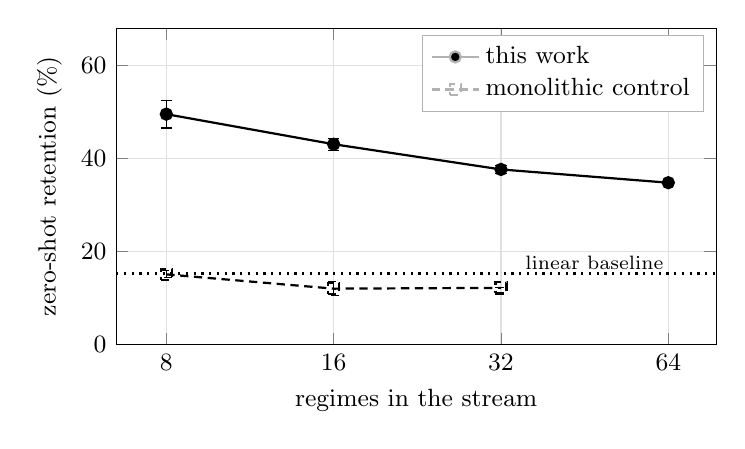
\begin{tikzpicture}
\begin{axis}[
  width=9.2cm, height=5.6cm,
  xmode=log, log basis x=2, xtick={8,16,32,64}, xticklabels={8,16,32,64},
  xlabel={regimes in the stream}, ylabel={zero-shot retention (\%)},
  ymin=0, ymax=68, xmin=6.5, xmax=78,
  ytick={0,20,40,60},
  grid=major, grid style={black!12},
  legend cell align=left,
  legend style={font=\small, draw=black!30, at={(0.98,0.98)}, anchor=north east},
  tick label style={font=\small}, label style={font=\small},
]
\addplot[thick, mark=*, mark size=2pt, error bars/.cd, y dir=both, y explicit]
  coordinates {(8,49.53) +- (0,2.98) (16,43.07) +- (0,1.31)
               (32,37.65) +- (0,0.78) (64,34.80) +- (0,0.28)};
\addlegendentry{this work}
\addplot[thick, densely dashed, mark=square, mark size=2pt,
         error bars/.cd, y dir=both, y explicit]
  coordinates {(8,15.10) +- (0,0.75) (16,12.03) +- (0,1.46) (32,12.20) +- (0,0)};
\addlegendentry{monolithic control}
\addplot[dotted, thick, domain=6.5:78, samples=2, forget plot] {15.30};
\node[anchor=west, font=\scriptsize] at (axis cs:34,17.6) {linear baseline};
\end{axis}
\end{tikzpicture}
\caption{Mode A. Bars are one standard deviation across seeds ($n=3$ at eight
and sixteen, $n=2$ at thirty-two and sixty-four for this work; $n=3$, $3$, $1$
for the control). The control sits at the level of a linear baseline without
sparse coding, so the task is not solvable by predicting frequent targets. The
sixty-four-regime control was not obtained: a single cell costs about nine
hours here and the run was lost.}
\label{fig:scale}
\end{figure}

Where a regime is identifiable from its own inputs, allocation retains
$49.53\%$, $43.07\%$ and $37.65\%$ of probed facts at eight, sixteen and
thirty-two regimes, against $15.10\%$, $12.03\%$ and $12.20\%$ for a monolithic
sparse-coded control of the same width: advantages of $+34.43$, $+31.04$ and
$+25.45$ points (Figure~\ref{fig:scale}). The advantage narrows as regimes
accumulate but does not close over the range we could measure. Both series
decline, and \S\ref{sec:scale} asks why ours does.

\subsection{Sharing the transform, privatising the readout}
\label{sec:sharing}

\begin{figure}[h]
\centering
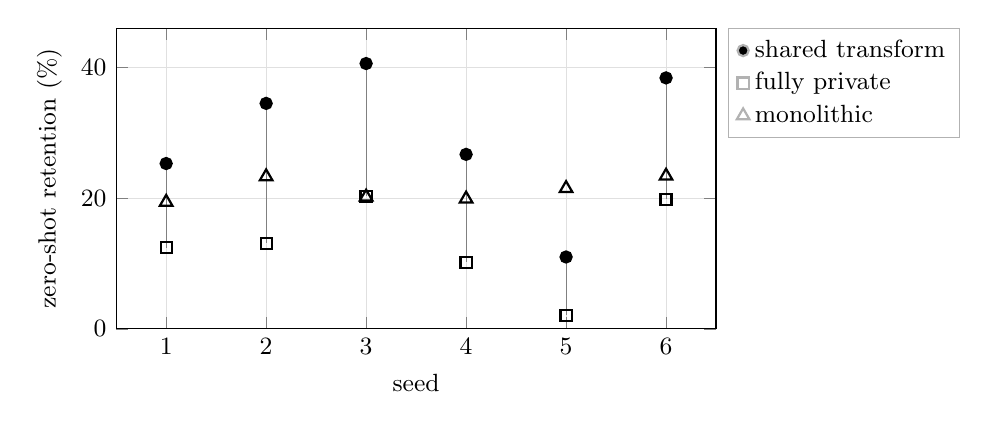
\begin{tikzpicture}
\begin{axis}[
  width=9.2cm, height=5.4cm,
  xlabel={seed}, ylabel={zero-shot retention (\%)},
  xtick={1,2,3,4,5,6}, xmin=0.5, xmax=6.5, ymin=0, ymax=46,
  grid=major, grid style={black!12},
  legend style={font=\small, draw=black!30, at={(1.02,1)}, anchor=north west},
  legend cell align=left,
  tick label style={font=\small}, label style={font=\small},
]
\addplot[thick, mark=*, mark size=2pt, only marks]
  coordinates {(1,25.3)(2,34.5)(3,40.6)(4,26.7)(5,11.0)(6,38.4)};
\addlegendentry{shared transform}
\addplot[thick, mark=square, mark size=2pt, only marks]
  coordinates {(1,12.4)(2,13.1)(3,20.3)(4,10.2)(5,2.1)(6,19.8)};
\addlegendentry{fully private}
\addplot[thick, mark=triangle, mark size=2.6pt, only marks]
  coordinates {(1,19.4)(2,23.3)(3,20.2)(4,19.9)(5,21.5)(6,23.4)};
\addlegendentry{monolithic}
\addplot[gray, forget plot] coordinates {(1,25.3)(1,12.4)};
\addplot[gray, forget plot] coordinates {(2,34.5)(2,13.1)};
\addplot[gray, forget plot] coordinates {(3,40.6)(3,20.3)};
\addplot[gray, forget plot] coordinates {(4,26.7)(4,10.2)};
\addplot[gray, forget plot] coordinates {(5,11.0)(5,2.1)};
\addplot[gray, forget plot] coordinates {(6,38.4)(6,19.8)};
\end{axis}
\end{tikzpicture}
\caption{Mode B, twelve regimes, per seed. Absolute retention varies by a
factor of nearly four across seeds ($11.0$ to $40.6$), which is why the paired
comparison is the one that carries weight: the vertical connectors are all the
same sign, $+8.9$ to $+21.4$ points, $6/6$. Against the monolithic control the
same comparison is $5/6$ and not established.}
\label{fig:share}
\end{figure}

\begin{table}[h]
\centering
\begin{tabular}{lcc}
\toprule
Mode B, twelve regimes, six seeds & zero-shot & paired difference \\
\midrule
Shared transform, private readouts & $\mathbf{29.42\%}$ & $+16.43$pp, 6/6, $p<0.001$ \\
Fully private & $12.98\%$ & --- \\
Monolithic & $21.28\%$ & $+8.13$pp, 5/6, $p=0.119$ \\
\bottomrule
\end{tabular}
\caption{Sharing the transform is established against the private
architecture. The advantage over the monolithic control is not.}
\end{table}

Sharing the \emph{readout} as well costs $27.50$ points. A common readout block
is updated on every write and therefore accumulates every regime's target
mapping, while Mode B is defined by the same $(e,r)$ pointing at different
targets per regime; it averages contradictions. The asymmetry of
\S\ref{sec:method} is thus confirmed from both sides, one by making the change
and the other by testing its opposite.

\subsection{Capacity follows content}
\label{sec:capacity}

\begin{table}[h]
\centering
\begin{tabular}{lccc}
\toprule
 & occupied rows & rows per class & accuracy \\
\midrule
Dense delta rule & $45056/45056$ ($100\%$) & $4096$ & $32.6\%$ \\
Sampled from emitted targets & $5918/45056$ ($\mathbf{13.1\%}$) & $\mathbf{538}$ & $33.8\%$ \\
\bottomrule
\end{tabular}
\caption{A $7.6\times$ reduction in occupied capacity at no cost in accuracy.}
\end{table}

One qualification belongs with this result rather than in the limitations. The
quantity capacity is supposed to follow is the union of distinct emitted
targets, and Heaps' law predicts that union to grow sublinearly in a
Zipf-distributed stream \citep{heaps1978information}. Our generator does not
produce that: the union measured at eight, sixteen, thirty-two and sixty-four
regimes is $273$, $534$, $1066$ and $2111$ distinct targets, or $34.2$, $33.4$,
$33.3$ and $33.0$ per regime --- flat, so the union grows \emph{linearly} in
regimes. Each regime samples its own entity and target pool, so there is little
shared vocabulary to amortise, and the sublinear growth that makes allocation
attractive on natural text is absent by construction. The reading this permits
is the narrow one: occupancy tracks emitted content rather than vocabulary
size. Whether that translates into sublinear capacity growth requires a source
with Heaps' law structure, which ours is not.

\subsection{Expansion does not disturb what is stored}
\label{sec:expansion}

Appending a class slice leaves every existing weight byte-identical and
\texttt{forward} bit-identical, asserted as a test rather than measured
statistically. A monolithic model cannot offer this: its capacity is the
sparse-coding width, and widening it changes the projection through which every
stored code was written.

\subsection{Cost per token is independent of context length}
\label{sec:cost}

\begin{figure}[h]
\centering
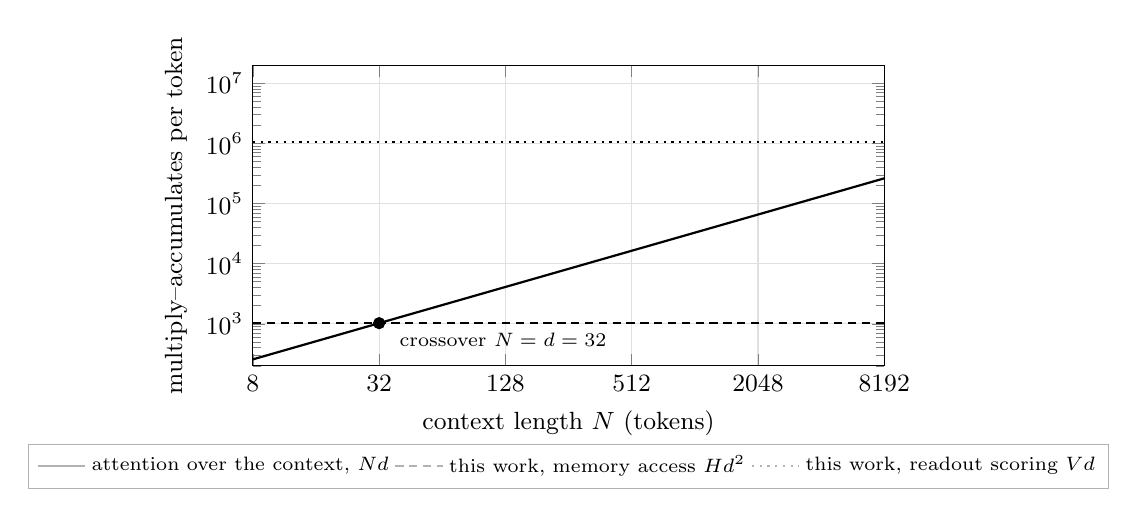
\begin{tikzpicture}
\begin{axis}[
  width=9.6cm, height=5.4cm, xmode=log, ymode=log, log basis x=2,
  xlabel={context length $N$ (tokens)},
  ylabel={multiply--accumulates per token},
  xmin=8, xmax=8192, ymin=200, ymax=20000000,
  xtick={8,32,128,512,2048,8192}, xticklabels={8,32,128,512,2048,8192},
  grid=major, grid style={black!12},
  legend style={font=\scriptsize, draw=black!30, at={(0.5,-0.26)}, anchor=north},
  legend columns=3, legend cell align=left,
  tick label style={font=\small}, label style={font=\small},
]
\addplot[thick, domain=8:8192, samples=2] {32*x};
\addlegendentry{attention over the context, $Nd$}
\addplot[thick, densely dashed, domain=8:8192, samples=2] {1024};
\addlegendentry{this work, memory access $Hd^2$}
\addplot[thick, dotted, domain=8:8192, samples=2] {1048576};
\addlegendentry{this work, readout scoring $Vd$}
\addplot[only marks, mark=*, mark size=2pt, forget plot] coordinates {(32,1024)};
\node[anchor=north west, font=\scriptsize] at (axis cs:36,1024) {crossover $N=d=32$};
\end{axis}
\end{tikzpicture}
\caption{Per-token cost at the configuration behind \S\ref{sec:modea}
($d=32$, $H=1$, $V=32768$). The memory access is flat in $N$ and crosses
attention at $N=d$; at $N=4096$ the ratio is $128\times$. The qualification is
the dotted line: the readout scores all $V$ rows, so it exceeds the memory
access by a factor of $1024$ and dominates the total. It too is flat in $N$ ---
the cost is constant in context length, but the constant is set by the dense
half. Making it follow occupancy instead is the first variant of
\S\ref{sec:variants}: a class holds $39$--$41$ occupied rows of the $32768$
scored.}
\label{fig:cost}
\end{figure}

Memory access costs $Hd^2$ per token regardless of sequence length, against
$Nd$ per token for dot-product attention over a context of $N$ tokens; the
crossover is at $N=d$ and the ratio is $128\times$ at $N=4096$
(Figure~\ref{fig:cost}). Against ourselves the reading is less flattering. In
the runs behind \S\ref{sec:modea}, activation is $1{,}049{,}600$ of
$269{,}547{,}520$ memory parameters per token, or $0.389\%$; but of that
activation the edge memory accounts for $1{,}024$ and the readout, scoring all
$V=32768$ rows, for $1{,}048{,}576$. The expert half is sparse and the readout
half is not, and the half that is not is a thousand times the larger. What is
constant in context length is the total; what sets that constant is the dense
half.

\section{Open questions}
\label{sec:open}

Every negative reading in this study that we examined closely turned out, at
least once, to be produced by the measurement rather than by the mechanism
(Appendix~\ref{app:invalidated}). We therefore report the following as
measurements whose interpretation is unsettled, rather than as properties of
the architecture.
\paragraph{Can the mechanism associate across a gap?}
\label{sec:longrange}

Nothing is carried between facts beyond a single-timescale context, so a cue
survives $(1-\rho)^{\text{gap}}$.

\begin{table}[h]
\centering
\begin{tabular}{ccc}
\toprule
gap & cue remaining & accuracy \\
\midrule
$1$ & $0.990$ & $10.10\%$ \\
$16$ & $0.851$ & $10.33\%$ \\
$64$ & $0.526$ & $8.40\%$ \\
$256$ & $0.076$ & $6.83\%$ \\
\bottomrule
\end{tabular}
\caption{Cue remaining is $(1-\rho)^{\text{gap}}$ at the context rate used.
Paired degradation from gap $1$ to gap $256$ is $+3.27$pp, 5/6 seeds,
$t(5)=3.81$, $p=0.013$. The location of the cliff was predicted from the
context rate before the run. Seeds 1--3 and 4--6 were run on different machines
at the same configuration and differ substantially in level ($5.1$--$9.0$
against $9.4$--$15.9$ at gap $1$), which is why the comparison is paired within
seed and the column means should not be read as a level.}
\end{table}

Exact association under constant memory is information-theoretically
unavailable, so the design question is what a lossy code should retain. A
multi-scale average answers \emph{which regime} and cannot answer \emph{which
item}. Placing context into the address recovers roughly a tenth of the gap and
costs lookup accuracy, consistent with content-only addressing being what
forbids association in the first place.

The evaluation itself is unfavourable to the mechanism, and we want that on
the record. Each run fixes a single gap, and a single gap is best served by
whichever single time constant happens to match it; a multi-scale context can
therefore show no advantage under this protocol by construction, because the
comparison is decided by the evaluation rather than by the code.

Under a mixed-gap protocol that cycles horizons within a run, the sign of the
effect changes: the strongest context gain we tried is worth $+0.67$pp on
average against no context in the address ($44.47\%\to45.13\%$, two seeds of
three in the favourable direction), where under a single fixed gap the same
setting bought $+0.40$pp at the long end while costing $0.47$pp at the short
one. We report this as a sign change and nothing more, and three facts about it
should be read alongside. The intermediate gain was \emph{negative}
($43.00\%$), so the response is not monotone in the amount of context; the
spread across seeds, $37.0$ to $52.4$ per cent, is an order of magnitude larger
than the effect; and three seeds cannot establish a difference of this size.
What it is consistent with is the protocol rather than the code having decided
the earlier comparison. We regard both protocols as
preliminary: a gap constructed in a synthetic stream fixes what has to be
carried and for how long, and cannot show what a real dependency structure
demands. Establishing this needs evaluation on natural language at scale, which
we have not done.

Whether this is a limit of the mechanism or of this particular probe is not
settled. Three earlier versions of the same measurement were invalid, each for
a different reason, and the fourth is the one reported here; placing context
into the address recovers roughly a tenth of the gap, which suggests the
addressing scheme rather than the context code may be the binding constraint.

\paragraph{Does multi-hop addressing ever pay?}

\begin{table}[h]
\centering
\begin{tabular}{cccc}
\toprule
hops & seeds & zero-shot & occupied rows \\
\midrule
$1$ & $2$ & $\mathbf{55.15\%}$ & $750$ \\
$2$ & $1$ & $46.00\%$ & $737$ \\
$3$ & $3$ & $29.63\%$ & $744$ \\
\bottomrule
\end{tabular}
\caption{Occupancy is the same to within $2\%$ while retention falls by half.
The seed counts are unequal and small, and the two-hop cell is a single run; on
the two seeds all three depths share, the ordering is the same ($54.2$, $56.1$
at one hop against $31.2$, $25.8$ at three). The under-training explanation is
excluded: writes per edge \emph{rise} with hops, from $3246$ to $9222$, because
each fact touches more edges.}
\end{table}

We do not conclude that depth is unnecessary, and the setup is narrow enough
that we could not. Multi-hop is the only form of depth this architecture has,
and it is depth in the transform rather than in the routing: hop $h+1$
transforms hop $h$'s output, but every hop selects its edge with the same fixed
copy of $p_0$, so the sequence of edges a fact visits is settled by its original
content. An earlier version of this comparison was taken while regime
separation had collapsed; the present one uses a single source, one scale, and a lookup task
whose targets are determined entirely by the current fact. A source that
rewards composition --- where an answer follows from chaining two stored
relations rather than retrieving one --- is exactly where combinatorial
addressing would be expected to pay, and we have not built one. What the table
shows is that paths cost accuracy when nothing requires a path.

\paragraph{Why does retention decline as regimes accumulate?}
\label{sec:scale}

\begin{figure}[h]
\centering
\begin{subfigure}[t]{0.48\textwidth}
\centering
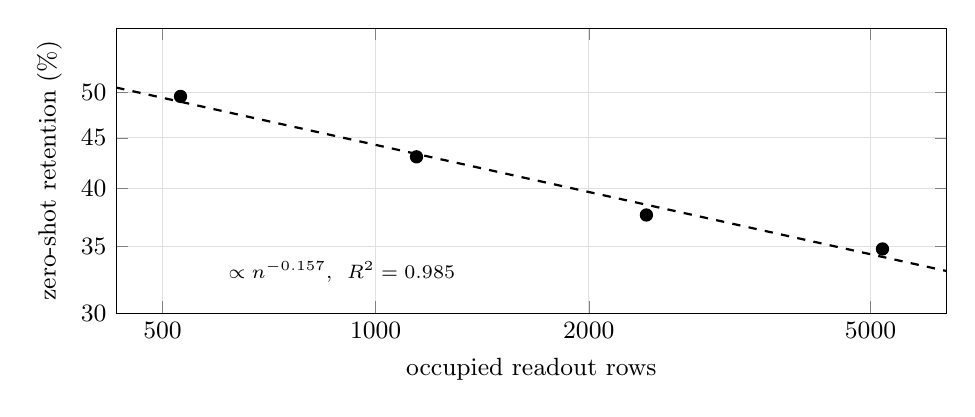
\begin{tikzpicture}
\begin{axis}[
  width=\textwidth, height=5.2cm, xmode=log, ymode=log,
  xlabel={occupied readout rows}, ylabel={zero-shot retention (\%)},
  xmin=430, xmax=6400, ymin=30, ymax=58,
  ytick={30,35,40,45,50}, yticklabels={30,35,40,45,50},
  xtick={500,1000,2000,5000}, xticklabels={500,1000,2000,5000},
  log ticks with fixed point,
  grid=major, grid style={black!12},
  tick label style={font=\small}, label style={font=\small},
]
\addplot[thick, dashed, domain=430:6400, samples=2, forget plot] {131.05*x^(-0.1571)};
\addplot[only marks, mark=*, mark size=2.2pt, forget plot]
  coordinates {(530,49.53)(1142,43.07)(2412,37.65)(5198,34.80)};
\node[anchor=south west, font=\scriptsize] at (axis cs:600,31.5)
  {$\propto n^{-0.157}$,\ \ $R^2=0.985$};
\end{axis}
\end{tikzpicture}
\caption{Retention against the inventory.}
\end{subfigure}
\hfill
\begin{subfigure}[t]{0.48\textwidth}
\centering
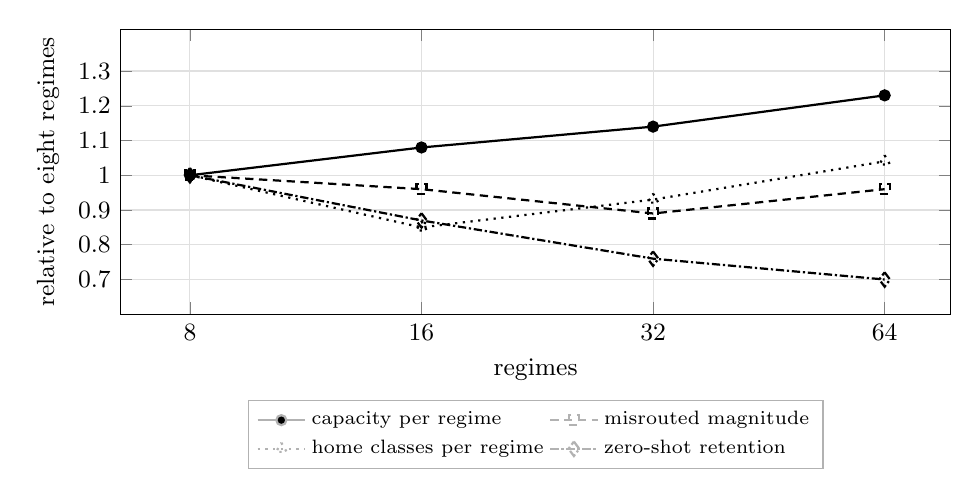
\begin{tikzpicture}
\begin{axis}[
  width=\textwidth, height=5.2cm,
  xmode=log, log basis x=2, xtick={8,16,32,64}, xticklabels={8,16,32,64},
  xlabel={regimes}, ylabel={relative to eight regimes},
  xmin=6.5, xmax=78, ymin=0.6, ymax=1.42,
  ytick={0.7,0.8,0.9,1.0,1.1,1.2,1.3},
  grid=major, grid style={black!12},
  legend style={font=\scriptsize, draw=black!30, at={(0.5,-0.30)}, anchor=north},
  legend columns=2, legend cell align=left,
  tick label style={font=\small}, label style={font=\small},
]
\addplot[thick, mark=*, mark size=1.8pt]
  coordinates {(8,1.00)(16,1.08)(32,1.14)(64,1.23)};
\addlegendentry{capacity per regime}
\addplot[thick, densely dashed, mark=square, mark size=1.8pt]
  coordinates {(8,1.00)(16,0.96)(32,0.89)(64,0.96)};
\addlegendentry{misrouted magnitude}
\addplot[thick, dotted, mark=triangle, mark size=2.2pt]
  coordinates {(8,1.00)(16,0.85)(32,0.93)(64,1.04)};
\addlegendentry{home classes per regime}
\addplot[thick, mark=diamond, mark size=2.6pt, densely dashdotted]
  coordinates {(8,1.00)(16,0.87)(32,0.76)(64,0.70)};
\addlegendentry{zero-shot retention}
\end{axis}
\end{tikzpicture}
\caption{Three candidates flat; retention not.}
\end{subfigure}
\caption{Three explanations for the decline are excluded, leaving one. Both
panels are normalised to the eight-regime value. \textbf{(b)} Capacity per
regime \emph{rises} ($66\to81$ occupied rows per regime), so this is not
starvation; misrouted write magnitude is flat ($57.0$, $54.7$, $51.0$, $55.0$
per cent), so it is not worsening interference; home classes per regime is flat
($0.75$, $0.64$, $0.70$, $0.78$), so separation does not degrade. Retention is
the only one of the four that moves. \textbf{(a)} The quantity it moves with is
the inventory the argmax must discriminate among, which grows $9.8\times$ over
the same range; against that inventory the decline is close to a power law,
$\propto n^{-0.157}$ with $R^2=0.985$ on four points. Note that the prediction
distribution does not collapse: distinct targets predicted rise from $47$ to
$57$ as accuracy falls, which is what distinguishes a discrimination failure
from a representational one. Four points and two to three seeds per point are
too few to fix an exponent; we read the figure as ruling three accounts out,
not as measuring a law.}
\label{fig:decline}
\end{figure}

Three explanations are excluded by the data (Figure~\ref{fig:decline}).
Capacity is supplied faster than linearly in regimes, so this is not
starvation. Misrouted write magnitude is flat, so it is not worsening
interference. Home classes per regime is flat, so separation does not degrade.
What remains is retrieval: the inventory of occupied readout rows --- the set
the argmax must discriminate among --- grows $9.8\times$ while accuracy falls
to $0.70\times$, and distinct predictions rise from $47$ to $57$ rather than
collapsing.

These exclusions constrain the explanation without establishing it, and the
monolithic baselines beyond sixteen regimes are still running. We state the
retrieval account as the surviving candidate rather than as the finding.



\paragraph{Does directed forgetting reclaim anything?}
We cannot say. Every measurement we made of it is confounded. The earlier ones
ran while a per-domain snapshot keyed by ground truth was reaching the training
path, and the later one, which added capacity pressure so that a freed slice
would be worth something, ran while the allocation criterion was collapsing
every regime into a single class --- so there were no separate slices to
reclaim in the first place. We report no number for it, and note only that a
valid test requires contention between regimes for storage \emph{and} a working
allocator, which we did not have simultaneously.

\paragraph{Does acquiring a regime become cheaper as regimes accumulate?}
Later regimes do cost less per unit accuracy in our runs, but our measurement
staggers arrival, and arrival order is itself sufficient to produce the effect:
a regime arriving late enters a system whose transform and prototypes are
already shaped. Separating order from content requires a design we have not
run, so we leave the question open rather than answer it from a measurement
that cannot distinguish the two (Appendix~\ref{app:arrival}).

\paragraph{Is the decline with scale a power law?}
Over the measured range, retention falls as $n^{-\alpha}$ with $\alpha=0.157$
and $R^2=0.985$, $n$ being the number of occupied readout rows
(Figure~\ref{fig:decline}a). Four points and two to three seeds per point
cannot distinguish a power law from any other slowly decaying form, so we
report the fit as a compact summary of the range measured and not as a law.
Whether the exponent is a property of the mechanism, and whether stronger
addressing rather than more capacity moves it, is measurable without new
machinery: the hierarchical variant of \S\ref{sec:variants} predicts it should
fall.

\paragraph{What should a constant-memory context retain?}
Exact association across a gap is information-theoretically unavailable under
constant memory, so the design question is what to keep. A multi-scale average
answers \emph{which regime} and cannot answer \emph{which item}. Sparse
retention of salient items, or superposition with approximate unbinding
\citep{plate1995holographic,ba2016using}, keeps identity where an average
cannot.

\paragraph{Does the plasticity--stability frontier extend or shift?}

\begin{figure}[h]
\centering
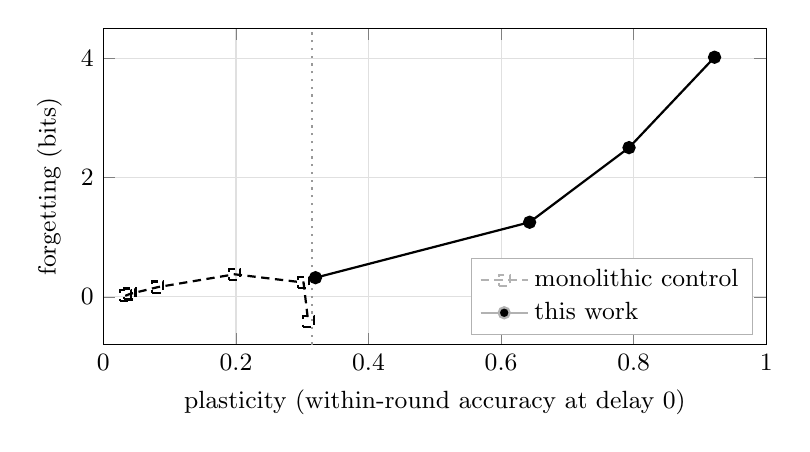
\begin{tikzpicture}
\begin{axis}[
  width=10cm, height=5.6cm,
  xlabel={plasticity (within-round accuracy at delay $0$)},
  ylabel={forgetting (bits)},
  xmin=0, xmax=1.0, ymin=-0.8, ymax=4.5,
  grid=major, grid style={black!12},
  legend style={font=\small, draw=black!30, at={(0.98,0.03)}, anchor=south east},
  legend cell align=left,
  tick label style={font=\small}, label style={font=\small},
]
\addplot[thick, mark=square, mark size=2pt, densely dashed]
  coordinates {(0.033,0.017)(0.040,0.049)(0.082,0.163)(0.198,0.378)
               (0.302,0.240)(0.309,-0.418)};
\addlegendentry{monolithic control}
\addplot[thick, mark=*, mark size=2pt]
  coordinates {(0.320,0.321)(0.643,1.250)(0.793,2.500)(0.922,4.014)};
\addlegendentry{this work}
\draw[black!40, dotted, thick] (axis cs:0.3145,-0.8) -- (axis cs:0.3145,4.5);
\end{axis}
\end{tikzpicture}
\caption{Each point is one learning rate, two or three seeds, Mode B at twelve
regimes; the rate sweeps $\eta\in\{0.1,\dots,30\}$ for the control and
$\{0.1,\dots,3\}$ for ours. The two arms do not overlap in plasticity at all:
the control saturates at $0.309$ and ours starts at $0.320$, either side of
the dotted line. Nothing about
frontier \emph{position} can be read from disjoint supports, which is why we
report reachability only. Two features are worth stating rather than
smoothing over: our forgetting grows steeply across our own range, $0.32$ to
$4.01$ bits, so the high-plasticity end is not free; and the control's
highest-rate cell has \emph{negative} forgetting, which we do not have an
account for and treat as a sign that the control is unstable there rather than
as a stability result.}
\label{fig:pareto}
\end{figure}

The frontier traced by our mechanism and that traced by the monolithic control
do not overlap in plasticity at all (Figure~\ref{fig:pareto}), so at present
only reachability can be compared, not position. Making the comparison possible
needs a regime in which both arms operate at the same plasticity, and we did
not construct one.

\section{Discussion}

\subsection{Why exact context cannot be cheap}

To associate any point in a stream with any other exactly, a system must be
able to answer for an arbitrary pair, which requires either retaining every
state and comparing against them --- $O(N)$ memory and $O(N)$ work per query
--- or precomputing the pairs, $O(N^2)$ in total. Self-attention pays exactly
this and buys exactness within its window in return
\citep{vaswani2017attention}. The cost is not an implementation artefact; it is
what pairwise access costs.

Under constant memory the question changes. Once the stream is longer than what
the memory can hold distinctly, some pairs must become unanswerable, and the
design decision is which ones. This is the same shape of decision that
continual learning already forces on the weights: bounded capacity against an
unbounded stream means something is given up, and methods differ in what
\citep{kirkpatrick2017overcoming,rusu2016progressive}. Our mechanism extends
that choice to the context.

\subsection{A fuzzy background instead of a transcript}

The position we take, and the one we find natural given the biological case, is
that a learner does not need a transcript of its context. A slowly varying
state that says \emph{what kind of situation this is} can serve as an anchor
for retrieval, leaving the identity of individual past items unrecoverable. Our
context is exactly that: an exponential summary matched against prototypes,
which conditions retrieval without recording what occurred.

Our measurements track this division cleanly. The mechanism answers ``which
regime'' well --- regimes separate, and retention exceeds the monolithic
control by $25$ to $34$ points --- and fails at ``which item occurred'' as soon
as a cue must survive a gap (\S\ref{sec:longrange}). That is the anchor working
as an anchor and failing as a record, which is what it is.

We do not claim this is the only division, or the best one. At least four
alternatives are available and differ in what they keep: sparse retention of a
few salient items keeps identity and discards time; superposition with
approximate unbinding keeps many items at graceful degradation
\citep{plate1995holographic}; outer-product fast weights keep pairs at a
capacity that scales with $d^2$ \citep{ba2016using,schlag2021linear}; and a
hybrid in which a fuzzy anchor selects a slice while a small exact buffer
covers the recent past would give up long-range exactness only. Which of these
is right is an empirical question we have not settled, and the answer may well
depend on what the stream is.

\subsection{Where this leaves three familiar problems}

\paragraph{Catastrophic forgetting.}
Allocation does not solve interference so much as convert it. Where a shared
representation loses old material as new material overwrites it
\citep{mccloskey1989catastrophic}, storage that is separated by regime removes
that channel and substitutes another: retrieval among a growing inventory. The
exchange rate looks favourable in our measurements --- confusable stored targets
grow $9.8\times$ while retention falls to $0.70\times$, and the distinct
predictions made rise rather than collapse --- but it is a substitution, not a
removal, and the cost reappears as scale.

The stronger reason to prefer it is not the rate but the shape of the two
failures. Interference in a shared representation
is destructive and open-ended: material that is overwritten is gone, and the
only remedies are more capacity or less learning. Retrieval difficulty is
non-destructive and sub-proportional: the material is still stored, merely
harder to find, and a tenfold larger inventory cost us thirty per cent of
retention. More importantly the two differ in what can be done about them.
Interference is answered only by spending parameters; retrieval difficulty is
answered by addressing better, which is a design axis rather than a budget.

That said, an exponent of roughly $0.16$ compounds, and a mechanism whose
retention decays with everything it has ever learned would not scale. Several
remedies follow directly from the diagnosis, and we list them in order of how
directly they attack the measured quantity, which is the number of candidates a
retrieval must discriminate among.

\begin{enumerate}
  \item \emph{Bound the scored set.} Inference currently scores all $V$ rows of
  the live slice while a class holds $39$--$41$ occupied rows. Scoring only
  occupied rows makes the candidate count follow content directly, which is the
  quantity in the exponent (\S\ref{sec:variants}).
  \item \emph{Shard the memory.} A coarse router over several independent
  memories, each with its own allocator, keeps any one inventory bounded while
  total capacity grows with the number of shards --- a mixture of experts whose
  experts are memories rather than layers
  \citep{shazeer2017outrageously,fedus2022switch}. Growth then adds shards
  rather than enlarging a single candidate set, so the exponent becomes a
  property of shard size instead of a property of everything ever learned. The
  cost is a second routing decision that can be wrong, and the open question is
  whether material that belongs to two shards must be duplicated.
  \item \emph{Address hierarchically.} Within a shard, a coarse code selecting a
  slice and a fine code over that slice's own targets makes discrimination
  logarithmic in the inventory rather than linear, at the cost of a coarse-level
  error being unrecoverable at the fine level (\S\ref{sec:variants}).
  \item \emph{Grow the code with the inventory.} Discriminating $N$ items needs
  a code whose capacity keeps pace; letting $d$ grow like $\log N$ would hold
  the exponent at the price of memory per row and of the byte-identical
  expansion property, since widening the code changes existing rows.
  \item \emph{Merge redundant slices.} If allocation over-splits, inventory
  reflects duplicates rather than distinct content. Consolidating slices whose
  similarity profiles coincide would keep the inventory a measure of what is
  actually distinct.
  \item \emph{Sample negatives adversarially.} Discrimination is currently
  trained against negatives drawn from a regime's own emitted targets. Drawing
  them from the current nearest confusables instead spends the code where
  collisions actually occur.
\end{enumerate}

The first two are the ones we would try first, and the second is the one that
changes the asymptote rather than the constant.

\paragraph{Lost in the middle.}
Attention degrades on material by its position in the context
\citep{liu2024lost}. Content addressing has no position term at all: a fact
stored early is reached by the same hash as one stored late, so retrieval
carries no positional decay. What decays instead is regime identification,
because the context summary is recency-weighted, and what degrades with load is
retrieval, because the inventory grows. The degradation is therefore moved off
position and onto inventory and recency, which is a different failure surface
rather than a smaller one --- a prediction that is testable directly, and that
we have not tested.

\paragraph{Plasticity and stability.}
We do not beat the frontier. Our mechanism and the monolithic control barely
overlap in plasticity: the control saturates near $0.31$ while ours spans
$0.32$ to $0.92$, so at present the honest statement is about reachability, not
position. Whether the frontier is extended or merely shifted requires a regime
where both operate, which we did not construct.

\subsection{What this is not for, and what it might be for}

A statically trained model, evaluated as a static tool, remains the accuracy
ceiling. It is trained to convergence over a fixed corpus with many passes; a
single-pass online memory will not match it on a benchmark drawn from that same
corpus, and we do not suggest otherwise. For answering ordinary questions from
knowledge fixed at training time, the static model is the right instrument and
this one is not.

The case for a mechanism like ours is different in kind: acceptable accuracy
combined with the ability to keep working. We would also note that accuracy on
a fixed source is a narrow proxy. It measures what a model knows at the moment
it was frozen, not what it can absorb afterwards, not what it costs to keep
running, and not what happens after weeks of operation --- none of which a
static benchmark is constructed to reveal. The properties measured here point
at settings where those are the binding constraints.

\emph{Sessions measured in weeks.} Per-token cost does not grow with context
and there is no cache to retain, so an agent can run for as long as the task
lasts rather than as long as a window allows. What it absorbed on the first day
is stored rather than scrolled out.

\emph{Embodied and IoT settings.} A robot or sensor node meets regimes that
were not enumerated in advance and receives them once, in order, without
labels. Allocation from the stream and single-pass writing match that shape;
retraining cycles do not.

\emph{Edge and green deployment.} Context access is $Hd^2$ per token
independently of history, and a write touches one slice and a handful of rows.
The cost profile is close to flat in the length of the deployment, which is the
quantity that dominates energy over a long-running installation.

\emph{Absorbing new domains after deployment.} Capacity appends without
disturbing what is stored, so a fielded model can take on a new domain without
a retraining cycle. The exactness matters more than the magnitude: one can
state that adding capacity did not change existing behaviour, rather than
measure that it changed little.

\emph{Targeted deletion, and interpretability more broadly.} A regime occupies
identifiable slices, so removing one is a local operation rather than a
retraining problem --- the natural test of the same structure that makes
expansion non-destructive, and one we have not run. The same property supports
weaker but broader questions: which slice serves this material, what did this
write change, what would removing this regime cost. A learned router gives no
comparable account of itself, and a dense model gives none at all. We think
this is the more interesting direction of the two, since deletion is one query
among many that an addressable, inspectable store can answer.

\emph{Long-tail material.} Capacity follows emitted content rather than
vocabulary size, so rare items occupy their own rows instead of being averaged
into frequent neighbours.

\subsection{Fabrication}

We did not measure hallucination and make no claim about rates. But three
structural properties bear on it and are worth stating, since each is a
consequence of the architecture rather than of tuning.

Training and inference are not separate modes: the same forward path writes and
reads, and what a query returns is what some slice holds. There is no
generation stage distinct from retrieval in which content can be composed that
was never stored.

Regimes occupy separate readout slices, so an answer is produced from the slice
the context selected. Blending material across domains --- one plausible route
to a confident wrong answer --- is limited by the same separation that limits
interference, rather than by a penalty term.

Sparse occupancy makes absence representable. A class holds tens of occupied
rows out of tens of thousands, so ``nothing here scores well'' is a state the
mechanism can be in, which a dense readout normalised over the full vocabulary
cannot easily express. Whether this translates into calibrated abstention is
untested and would be the obvious experiment.

\subsection{On whether growing capacity is disqualifying}

Expansion invites the objection that a method which adds parameters has not
solved anything. We think the objection is right about unbounded growth and
wrong as a general principle, and the biological case is instructive on the
distinction. A brain does not hold its knowledge in a fixed parameter vector:
connectivity is combinatorial, signalling is graded rather than discrete, and
the number of distinguishable synaptic states is correspondingly large. A
system with that much effective capacity can afford to allocate in proportion
to content, because content is small relative to what it can hold.

Digital parameters are finite and discrete, so the same strategy is only
tenable if per-shard inventory is bounded --- which is the argument for
sharding above, and the reason we regard unbounded growth in a single memory as
a defect to be fixed rather than a property to be defended. What the biological
case does suggest is that allocation proportional to content is not
disqualifying in itself. What must be bounded is not the total, but the number
of things any single retrieval has to discriminate among.

\section{Architectural variants worth trying}
\label{sec:variants}

Each variant below targets a specific measurement in this paper rather than a
general intuition.

\paragraph{Bound scoring to the emitted rows.}
Inference scores all $V$ rows of the live readout slice, while a class holds
$39$--$41$ occupied rows against a vocabulary of $32768$. Restricting the
argmax to rows the class has emitted, with the remainder contributing a
constant, would cut inference cost by nearly three orders of magnitude and
would make the activation figure of \S\ref{sec:cost} sparse in both halves
rather than only in the expert half. Nothing about the mechanism resists this;
it is unimplemented, not difficult.

\paragraph{Address hierarchically to bound the candidate set.}
The decline with scale tracks the number of confusable stored items rather than
capacity, misrouting or separation (\S\ref{sec:open}). If that account is
right, the fix is not more capacity but a smaller candidate set at retrieval:
a coarse regime code selecting a slice, then a within-slice code over that
regime's own targets, so that discrimination is against tens of alternatives
rather than thousands. This predicts that the exponent $\alpha$ should fall
with the depth of the addressing hierarchy, which is directly testable.

\paragraph{Add a term that stores pairs.}
A smoothed context can report which regime is active and cannot report which
item occurred, so no amount of extra timescales will support association across
a gap. An outer-product term, $M \leftarrow \lambda M + p_t \otimes p_{t-\Delta}$
retrieved as $Mp$, stores pairs recoverably at a capacity that scales with
$d^2$ \citep{ba2016using,schlag2021linear}, and is the same algebraic object as
the edge transform already present. The open question is whether it can sit
alongside content addressing without dissolving the stability that content
addressing provides.

\paragraph{Give the router a learned residual.}
The fixed random hash buys routing consistency of $1.000$ and forgoes load
balancing and learned specialisation. A learned correction added to the key,
small enough that a fact's destination remains stable within a regime, would
recover part of what a gated mixture of experts gets from its router
\citep{shazeer2017outrageously} without giving up the property that makes
expansion non-destructive.

\paragraph{Let the address compose, not only the value.}
The value path already composes: hop $h+1$ transforms hop $h$'s output and
gradients flow along the walked chain. What repeats is the \emph{address} ---
every hop selects its edge with the same fixed copy of $p_0$, so the sequence
of edges a fact visits is settled before the walk begins.

We implemented the obvious remedy, copying the transformed payload into the
routing key after each hop so that hop $h+1$ selects from hop $h$'s output, and
it makes matters worse. Within its own configuration, which uses a larger ring
than the multi-hop table above and is therefore not directly comparable to it,
accuracy falls from $51.43\%$ to $41.03\%$ at two hops and from $35.10\%$ to
$22.83\%$ at three, so the gap to a single hop widens rather than closes. The
reason is visible in the same run. Routing consistency, which the fixed key
guarantees at $1.000$, falls to $0.875$ at two hops and $0.740$ at three: a
fact's path now depends on weights that move, so an eighth and then a quarter
of probed facts no longer reach where training left them. The loss tracks the
depth, which is what one would expect if it compounds along the walk rather
than being a fixed cost, and it outweighs whatever composition buys. Whether a source that
genuinely requires chaining two stored relations would reverse the balance is
untested --- on a lookup whose target is fixed by the current fact there is
nothing for a composed path to find --- so this settles the version we tried
rather than the idea.

\paragraph{A note on tokenisation.}
We recommend against subword tokenisation for this architecture. Byte-pair
encoding is designed to flatten the frequency distribution, and this mechanism
depends on that distribution in two places: allocation splits a class when its
similarity dispersion rises, which requires regimes to differ in what they
emit, and capacity follows the count of distinct emitted targets, which
requires a target to be a unit rather than a sequence. A rare entity split into
several frequent subwords loses its identity twice over --- its payload becomes
a sum of common pieces, which collides in the content hash with every other
entity sharing those pieces, and its target becomes a sequence with no single
row to occupy. The long tail is exactly where a continual learner has something
to gain, and subword vocabularies are built to spend it. A word- or
entity-level vocabulary, or any tokenisation that keeps rare units intact,
preserves both the Zipf structure the allocator reads and the one-target-one-row
correspondence the capacity argument relies on.

\section{Limitations}

Results are on a synthetic relational source; no natural-language corpus is
evaluated, and a stream we constructed fixes what has to be learned and what
can be shared, which is precisely what a real corpus would decide for us.

The monolithic control is established at eight, sixteen and thirty-two regimes,
with one seed at thirty-two and none at sixty-four; our own cells at thirty-two
and sixty-four have two seeds each. The comparison is not parameter-matched in
either direction. At eight regimes the control holds a $512\times32768$
readout, $16.8$M weights, while our mechanism allocated $10$, $11$ and $13$
class slices across the three seeds --- $327{,}680$ to $425{,}984$ rows, $10.5$M
to $13.6$M weights --- of which $523$ to $538$ rows, about $17$K weights, are
occupied. These are two models of comparable width and different size, so the
occupancy figures describe our mechanism and are not a like-for-like efficiency
claim against the control.

Cost comparisons between the dense and sampled write paths are not
commensurable, because write magnitude accumulates over a different number of
rows in each. The private and shared arms likewise differ in parameter count,
which strengthens the accuracy comparison between them but confounds any
comparison of their costs.

Sample sizes are small throughout: six seeds for the sharing result, three for
most others, one for the largest control. Several effects in this study
weakened or reversed between three seeds and six, so single-digit seed counts
should be read accordingly.

Whether acquiring a regime becomes cheaper as regimes accumulate is not settled
here: our measurement staggers arrival, and arrival order alone can produce the
effect (Appendix~\ref{app:arrival}).

\section{Conclusion}

Content addressing with on-demand allocation buys a large advantage where
regimes are distinguishable, a capacity footprint that follows emitted content,
and a per-token cost independent of context length, without disturbing what is
already stored. The same commitment that makes storage
stable --- addressing by content alone --- is what prevents association across a
gap, and the cost of that trade is measured here rather than asserted.

\appendix

\section{Measurements invalidated during this study}
\label{app:invalidated}

Six measurements were invalidated after collection and re-run. Three were
probe-side leaks in which a per-domain snapshot keyed by ground truth handed the
mechanism the regime identity it was meant to infer. One was the allocation
criterion of \S\ref{sec:allocation} in an earlier form, which compared novelty
against a global running distribution and collapsed every regime into a single
class at scale, voiding the savings, capacity and multi-hop measurements taken
under it. One was a parser that scanned past the results table into a table with
the same column count and reported $54.2\%$ as $100.00\%$.

Each was caught by a contradiction between statistics rather than by reading
code: a count that disagreed with another count, a diagnostic that printed
nothing, an accuracy that could not coexist with its own exposure figures. The
instruments that survived --- write locality by time since regime change,
occupancy against emitted content, allocation timing against regime boundaries
--- are reported alongside the results because they are what made the failures
visible.

\section{Arrival order and the cost of a late regime}
\label{app:arrival}

Measuring whether a later regime is cheaper to acquire requires staggered
arrival, and staggering introduces a confound we record here for the benefit of
anyone running the same measurement.

\begin{table}[h]
\centering
\begin{tabular}{lcc}
\toprule
 & shared transform & private \\
\midrule
Mode A, staggered arrival & $0.754$ & $0.820$ \\
Mode B, disjoint targets, staggered arrival & $0.442$ & $0.505$ \\
Mode A, no staggering (index only) & $1.199$ & $1.207$ \\
\bottomrule
\end{tabular}
\caption{Cost of the late regimes relative to the early ones; below one means
a late regime is cheaper. Three seeds per control.}
\end{table}

Mode B's targets are disjoint across regimes by construction, so nothing there
can be amortised, yet the ratio is lower than in Mode A. Removing the
staggering removes the effect. A regime arriving late therefore benefits from
entering an already-shaped system, independently of whether it shares content
with its predecessors, and a ratio below one cannot on its own be read as
amortisation.

\begin{thebibliography}{99}

\bibitem[Aljundi et al.(2019)]{aljundi2019task}
R.~Aljundi, K.~Kelchtermans, and T.~Tuytelaars.
\newblock Task-free continual learning.
\newblock In \emph{CVPR}, 2019.

\bibitem[Ba et al.(2016)]{ba2016using}
J.~Ba, G.~Hinton, V.~Mnih, J.~Z. Leibo, and C.~Ionescu.
\newblock Using fast weights to attend to the recent past.
\newblock In \emph{NeurIPS}, 2016.

\bibitem[Benna and Fusi(2016)]{benna2016computational}
M.~K. Benna and S.~Fusi.
\newblock Computational principles of synaptic memory consolidation.
\newblock \emph{Nature Neuroscience}, 2016.

\bibitem[De Lange et al.(2021)]{delange2021continual}
M.~De~Lange, R.~Aljundi, M.~Masana, S.~Parisot, X.~Jia, A.~Leonardis,
  G.~Slabaugh, and T.~Tuytelaars.
\newblock A continual learning survey: Defying forgetting in classification
  tasks.
\newblock \emph{IEEE TPAMI}, 2021.

\bibitem[Fedus et al.(2022)]{fedus2022switch}
W.~Fedus, B.~Zoph, and N.~Shazeer.
\newblock Switch transformers: Scaling to trillion parameter models with simple
  and efficient sparsity.
\newblock \emph{JMLR}, 2022.

\bibitem[French(1999)]{french1999catastrophic}
R.~M. French.
\newblock Catastrophic forgetting in connectionist networks.
\newblock \emph{Trends in Cognitive Sciences}, 1999.

\bibitem[Fusi et al.(2005)]{fusi2005cascade}
S.~Fusi, P.~J. Drew, and L.~F. Abbott.
\newblock Cascade models of synaptically stored memories.
\newblock \emph{Neuron}, 2005.

\bibitem[Heaps(1978)]{heaps1978information}
H.~S. Heaps.
\newblock \emph{Information Retrieval: Computational and Theoretical Aspects}.
\newblock Academic Press, 1978.

\bibitem[Kanerva(1988)]{kanerva1988sparse}
P.~Kanerva.
\newblock \emph{Sparse Distributed Memory}.
\newblock MIT Press, 1988.

\bibitem[Kanerva(2009)]{kanerva2009hyperdimensional}
P.~Kanerva.
\newblock Hyperdimensional computing: An introduction to computing in
  distributed representation with high-dimensional random vectors.
\newblock \emph{Cognitive Computation}, 2009.

\bibitem[Kirkpatrick et al.(2017)]{kirkpatrick2017overcoming}
J.~Kirkpatrick, R.~Pascanu, N.~Rabinowitz, J.~Veness, G.~Desjardins, A.~A. Rusu,
  K.~Milan, J.~Quan, T.~Ramalho, A.~Grabska-Barwinska, et~al.
\newblock Overcoming catastrophic forgetting in neural networks.
\newblock \emph{PNAS}, 2017.

\bibitem[Liu et al.(2024)]{liu2024lost}
N.~F. Liu, K.~Lin, J.~Hewitt, A.~Paranjape, M.~Bevilacqua, F.~Petroni, and
  P.~Liang.
\newblock Lost in the middle: How language models use long contexts.
\newblock \emph{TACL}, 2024.

\bibitem[McCloskey and Cohen(1989)]{mccloskey1989catastrophic}
M.~McCloskey and N.~J. Cohen.
\newblock Catastrophic interference in connectionist networks: The sequential
  learning problem.
\newblock \emph{Psychology of Learning and Motivation}, 1989.

\bibitem[Parisi et al.(2019)]{parisi2019continual}
G.~I. Parisi, R.~Kemker, J.~L. Part, C.~Kanan, and S.~Wermter.
\newblock Continual lifelong learning with neural networks: A review.
\newblock \emph{Neural Networks}, 2019.

\bibitem[Plate(1995)]{plate1995holographic}
T.~A. Plate.
\newblock Holographic reduced representations.
\newblock \emph{IEEE Transactions on Neural Networks}, 1995.

\bibitem[Rusu et al.(2016)]{rusu2016progressive}
A.~A. Rusu, N.~C. Rabinowitz, G.~Desjardins, H.~Soyer, J.~Kirkpatrick,
  K.~Kavukcuoglu, R.~Pascanu, and R.~Hadsell.
\newblock Progressive neural networks.
\newblock \emph{arXiv:1606.04671}, 2016.

\bibitem[Schlag et al.(2021)]{schlag2021linear}
I.~Schlag, K.~Irie, and J.~Schmidhuber.
\newblock Linear transformers are secretly fast weight programmers.
\newblock In \emph{ICML}, 2021.

\bibitem[Shazeer et al.(2017)]{shazeer2017outrageously}
N.~Shazeer, A.~Mirhoseini, K.~Maziarz, A.~Davis, Q.~Le, G.~Hinton, and J.~Dean.
\newblock Outrageously large neural networks: The sparsely-gated
  mixture-of-experts layer.
\newblock In \emph{ICLR}, 2017.

\bibitem[Vaswani et al.(2017)]{vaswani2017attention}
A.~Vaswani, N.~Shazeer, N.~Parmar, J.~Uszkoreit, L.~Jones, A.~N. Gomez,
  L.~Kaiser, and I.~Polosukhin.
\newblock Attention is all you need.
\newblock In \emph{NeurIPS}, 2017.

\bibitem[Yoon et al.(2018)]{yoon2018lifelong}
J.~Yoon, E.~Yang, J.~Lee, and S.~J. Hwang.
\newblock Lifelong learning with dynamically expandable networks.
\newblock In \emph{ICLR}, 2018.

\end{thebibliography}

\end{document}
